\documentclass{beamer}
\beamertemplatenavigationsymbolsempty
\usecolortheme{beaver}
\setbeamertemplate{blocks}[rounded=true, shadow=true]
\setbeamertemplate{footline}[page number]
%
\usepackage[utf8]{inputenc}
\usepackage[english,russian]{babel}
\usepackage{amssymb,amsfonts,amsmath,mathtext}
\usepackage[]{algorithmic}
\usepackage{subfig}
\usepackage[all]{xy} % xy package for diagrams
\usepackage{array}
\usepackage{tikz}
\usepackage{multicol}% many columns in slide
\usepackage{hyperref}% urls
\usepackage{hhline}%tables
\usepackage{biblatex}
% Your figures are here:
\graphicspath{ {fig/} {../fig/} }
\usepackage{graphicx}
\usepackage{subcaption}
\usepackage{wrapfig}
\usepackage{amsmath}
\usepackage{caption}
\captionsetup{labelformat=empty}
\usepackage{subfigure}
\newcommand\normx[1]{\left\Vert#1\right\Vert}

\newcommand\myfootnote[1]{%
  \tikz[remember picture,overlay]
  \draw (current page.south west) +(1in + \oddsidemargin,0.5em)
  node[anchor=south west,inner sep=0pt]{\parbox{\textwidth}{%
      \rlap{\rule{10em}{0.4pt}}\raggedright\scriptsize \textit{#1}}};}

%----------------------------------------------------------------------------------------------------------
\title[\hbox to 56mm{Векторное представление моделей}]{Методы векторного представления глубоких генеративных моделей}
\author[М.\,А. Никитина]{Мария Александровна Никитина}
\institute{Московский физико-технический институт}
\date{\footnotesize
\par\smallskip\emph{Кафедра:} Интеллектуальный анализ данных
\par\smallskip\emph{Научный руководитель:} кандидат ф.-м. наук О.\,Ю.~Бахтеев
\par\smallskip\emph{Научный консультант:} А.\,Ю.~Бишук
\par\bigskip\small 2024}
%----------------------------------------------------------------------------------------------------------
\begin{document}
%----------------------------------------------------------------------------------------------------------
\begin{frame}
\thispagestyle{empty}
\maketitle
\end{frame}
%-----------------------------------------------------------------------------------------------------
\begin{frame}{Задача векторного описания генеративных моделей}
% \footnotesize
\begin{block}{Задача}
Задан набор генеративных моделей, описывающий разные выборки/генеральные совокупности данных. Требуется предложить метод векторного представления этих моделей, который будет представлять их статистические свойства.
\end{block}
\begin{block}{Требования}
\begin{enumerate}
    \item Расстояние между векторными представлениями моделей для близких выборок должно быть невелико (при условии, что сами модели хорошо их описывают)
    \item Модели, обученные на композиции/смеси выборок должны учитывать свойства всех выборок, входящих в смесь
\end{enumerate}
\end{block}
\end{frame}
%-----------------------------------------------------------------------------------------------------
\begin{frame}{Примеры возможных реализаций}
\begin{wrapfigure}{r}{0.35\textwidth}
  \vspace{-20pt}
  \begin{center}
    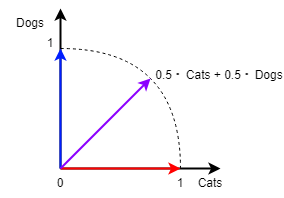
\includegraphics[width=0.4\textwidth]{Pictures/Classes.png}
  \end{center}
  \vspace{-20pt}
\end{wrapfigure}
1. Один из возможных вариантов: сумма векторных представлений моделей, полученных по датасетам $D_1$, $D_2$ должна приблизительно соответствовать векторному представлению датасета $D_1 + D_2$;

\bigskip

2. Вместо использования евклидового расстояния на векторных представлениях, использовать иерархию;

\bigskip

3.Представить модель как граф и работать с пространством графов.
\end{frame}
%----------------------------------------------------------------------------------------------------------
\begin{frame}{Описание эксперимента}
Для базового эксперимента берётся 3 наиболее удалённых класса из датасета CIFAR. Для поиска таких классов использовалось евклидово расстояние на ембеддингах, полученных из выходного слоя ResNet.

\begin{block}{Алгоритм}
\begin{enumerate}
    \item Случайное сэмплирование долей классов в датасете для $n$ моделей;

    \item Обучение $n$ моделей на соответствующих датасетах;

    \item Получение векторов из обученных моделей;

    \item Обучение энкодера на полученных моделях. Предсказание:
        \begin{enumerate}
            \item Вектора на части единичной сферы

            \item Расстояния между двумя моделями
        \end{enumerate}
\end{enumerate}
\end{block}
\end{frame}
%----------------------------------------------------------------------------------------------------------
\begin{frame}{Схема эксперимента}
\begin{figure}
    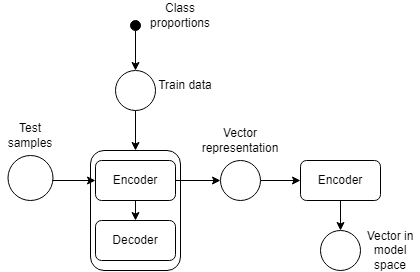
\includegraphics[width=1.0\linewidth]{Pictures/Model.png}
\end{figure}
\end{frame}
%----------------------------------------------------------------------------------------------------------
\begin{frame}{Возможные метрики}
\small
\begin{enumerate}
    \item Contrastive N-pair loss, где $\text{Encoder}(m_i) = \textbf{x}$, $\textbf{d}_i = \textbf{x}_i^+$, остальные элементы батча: $\textbf{x}_i^-$:

\[\mathcal{L}_{N-pair}(f) = - \log \frac{\exp(\textbf{x}^T \textbf{x}_i^+)}{\exp(\textbf{x}^T \textbf{x}_i^+) + \sum _{i=1}^{N-1} \exp(\textbf{x}^T\textbf{x}_i^-)};\]
    \item Угол между вектором модели $\text{Encoder}(m_i)$ и датасета $\textbf{d}_i$:

\[\mathcal{L}_{cos}(\text{Encoder}(m_i), \textbf{d}_i) = \cos(\text{Encoder}(m_i) \cdot \textbf{d}_i);\]

    \item Triplet loss:

\[\mathcal{L}_{Triplet} = \sum\limits_{x \in \chi}\max(0, ||\textbf{x} - \textbf{x}^+||_2^2 - ||\textbf{x} - \textbf{x}^-||_2^2 + \epsilon;\]

    \item MSE между $\text{Encoder}(m_i)$ и $\textbf{d}_i$:

\[\mathcal{L}_{MSE}(\text{Encoder}(m_i), \textbf{d}_i) = \|\text{Encoder}(m_i) - \textbf{d}_i)\|_2^2.\]
\end{enumerate}
\end{frame}
%----------------------------------------------------------------------------------------------------------
\begin{frame}{Результаты первого эксперимента}
\begin{wrapfigure}{r}{0.45\textwidth}
  \vspace{-30pt}
  \begin{center}
    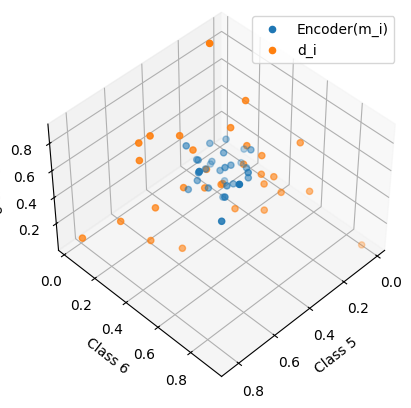
\includegraphics[width=0.5\textwidth]{Pictures/Encoder.png}
  \end{center}
  \vspace{-20pt}
\end{wrapfigure}

\textit{Способ представления модели}: среднее значение скрытого пространства автоэнкодера на тестовой выборке.

\bigskip

\textit{Метрика энкодера}: MSE

\bigskip

\textit{Проблемы}: Переобучение энкодера и неинформативность взятия среднего
\end{frame}
%----------------------------------------------------------------------------------------------------------
% \begin{frame}{Список литературы}
% \begin{thebibliography}{99} 
%     \footnotesize
    
%     \bibitem[Chuang, 2020]{p1}
%         Ching-Yao Chuang, Joshua Robinson, Lin Yen-Chen, Antonio Torralba, Stefanie Jegelkah (2020)
%         \newblock Debiased Contrastive Learning

%         \bibitem[Yang, 2022]{p2}
%         Yang, Jinyu and Duan, Jiali and Tran, Son and Xu, Yi and Chanda, Sampath and Chen, Liqun and Zeng, Belinda and Chilimbi, Trishul and Huang, Junzhou (2022)
%         \newblock Vision-Language Pre-Training with Triple Contrastive Learning

%        \bibitem[Chen2020SimCLR, 2020]{p3}
%         CTing Chen, Simon Kornblith, Mohammad Norouzi, Geoffrey Hinton (2020)
%         \newblock A Simple Framework for Contrastive Learning of Visual Representations

%     \bibitem[VQA, 2017]{p4}
%         Stanislaw Antol and Aishwarya Agrawal and Jiasen Lu and Margaret Mitchell and Dhruv Batra and C. Lawrence Zitnick and Devi Parikh (2017)
%         \newblock {VQA}: {V}isual {Q}uestion {A}nswering

%     \bibitem[schroff2015facenet, 2015]{p5}
%         Florian Schroff, Dmitry Kalenichenko, James Philbin (2015)
%         \newblock FaceNet: A Unified Embedding for Face Recognition and Clustering

% \end{thebibliography}
% \end{frame}
\end{document} 
